\section{Data}
\label{sec:data}

The dataset employed in this study comprises approximately 1,700 overlapping aerial images captured by drones at Texas A\&M AgriLife Research's Brazos Bottom Farm in Burleson County, Texas (headquarters at 30.549635N, 96.436821W) \cite{shi_2021_5089956}.

UAVs were operated by three distinct flight teams and were equipped with various sensors, auto-pilots, and stabilization systems. Most flights were conducted within two hours of solar noon. Flight and sensor parameters were configured to ensure the collection of high-quality images with sufficient overlap for mosaicking purposes and to minimize pixel smearing. For this case study, the images were captured with an X88 octocopter UAV at a typical flying altitude of 15-20 meters, employing a DJIP3-005 4K Camera with a resolution of 4000x3000 pixels.

Approximate locations of raw images (longitude, latitude, and altitude) were recorded by an onboard GPS; however, its accuracy is insufficient for direct georeferencing. Eight Ground Control Points (GCPs) were installed around the study area to facilitate accurate georeferencing, geometric correction, and co-registration of UAS data.

\subsection{Preprocessing}
\label{sec:preprocessing}

Significant long-term challenges related to data collection/processing and interpretation of the processed data need to be addressed before breeders can fully embrace these systems. Figure \ref{fig:dev_pipeline} illustrates the data processing workflow.

\begin{figure}[t!]
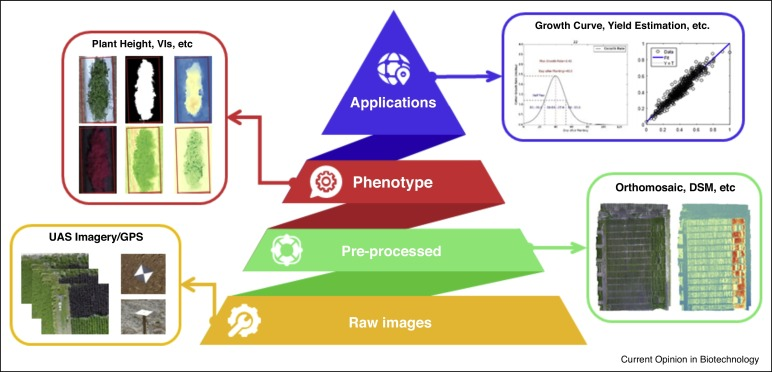
\includegraphics[width=\linewidth]{../images/dev_pipeline}
\caption{UAVs application development workflow. Adapted from \cite{jung2021potential}.}
\label{fig:dev_pipeline}
\end{figure}

No additional post-processing has been applied to the images as it has already been performed by the dataset's authors.

Since there is a time gap between the ground truth measurement and the generation of the DSM for height estimation, the ground truth values were averaged between the two.

GCPs are crucial for georeferencing the images and therefore for generating the orthomosaic. The 61x61cm concrete tiles were installed at the corners and interior locations of all UAVs' routes and were painted black, dark gray, and light gray ($\approx$ 10\%, 20\% and 40\% reflectance).

The provided GCPs coordinates were transformed from the EPSG:32614 (WGS 84 / UTM zone 14N) to the EPSG:4326 (WGS 84) coordinate reference system (CRS) using the QGIS software \footnote{QGIS is a free and open-source cross-platform desktop geographic information system application that supports viewing, editing, and analysis of geospatial data: \url{https://qgis.org/}}.

The GCPs coordinates were employed with the GCPEditorPro software \footnote{Ground Control Points Interface for OpenDroneMap software \url{https://github.com/uav4geo/GCPEditorPro}} to identify the tiles on the ground within the overlaying images collected by the UAVs. This process facilitated the georeferencing of the images, which was subsequently provided to the WebODM software to generate an orthomosaic of the field (Figure \ref{fig:orthomosaic}).

Finally, the plots were extracted from the orthomosaic using the Python Shapefile Library \footnote{PyShp reads and writes ESRI Shapefiles in pure Python: \url{https://github.com/GeospatialPython/pyshp}} by utilizing the shapefile provided in the dataset and then matched to the ground truth records to assign a height value to each of them.

\begin{figure}[b!]
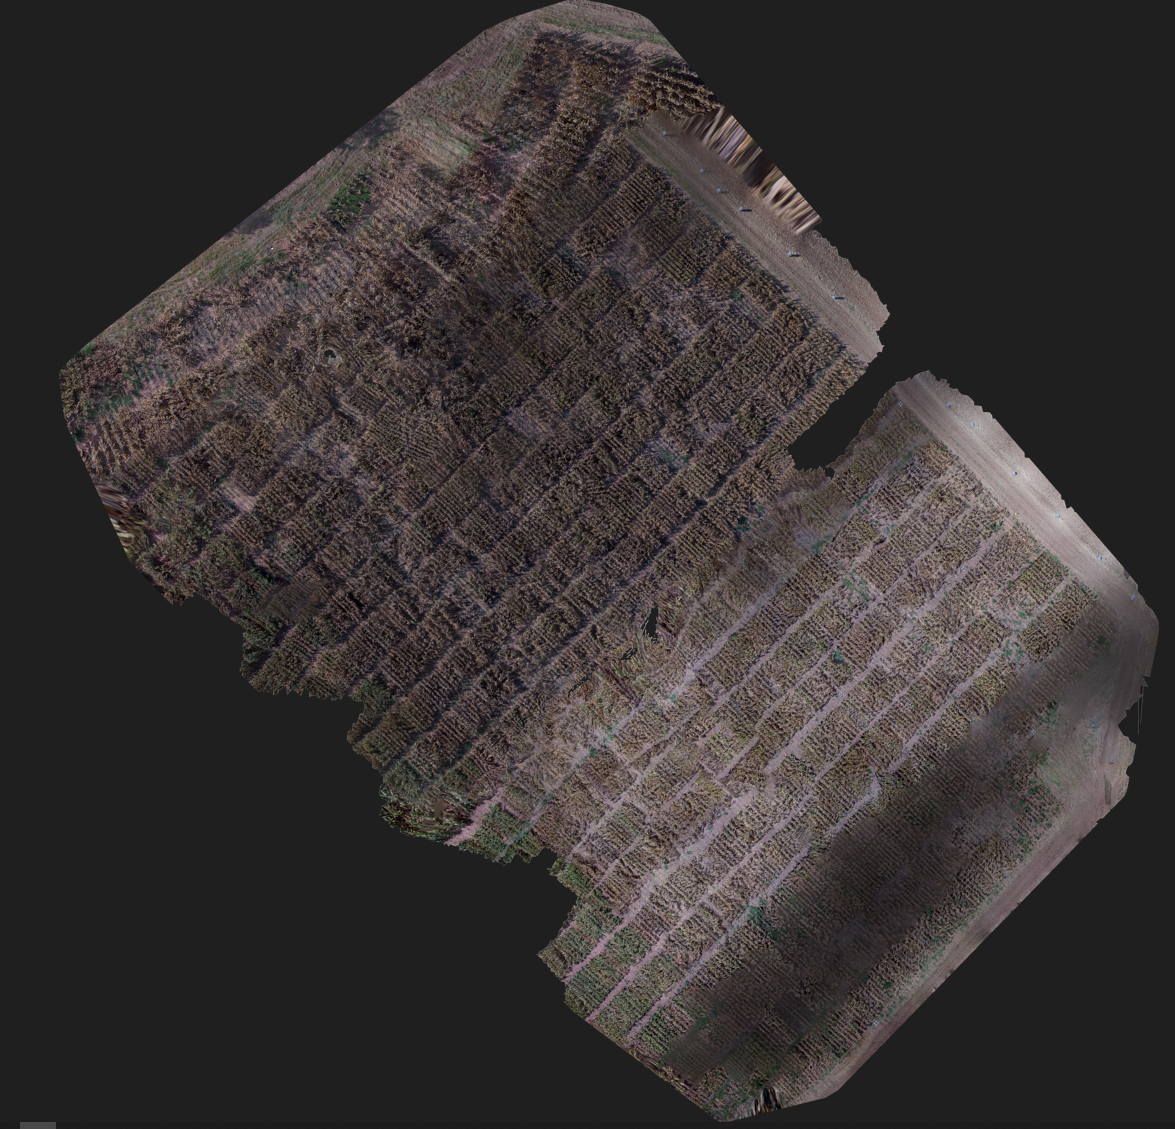
\includegraphics[width=\linewidth]{../images/orthomosaic}
\caption{Orthomosaic of the agricultural field. Produced with WebODM.}
\label{fig:orthomosaic}
\end{figure}